\clearpage\begingroup
\SourceLeaf{163}\HistoricalHead{158}{L}{PHYSIK.\quad BRIEFWECHSEL.}
\newcommand{\DioptrikLetterFifteenDiagram}{%
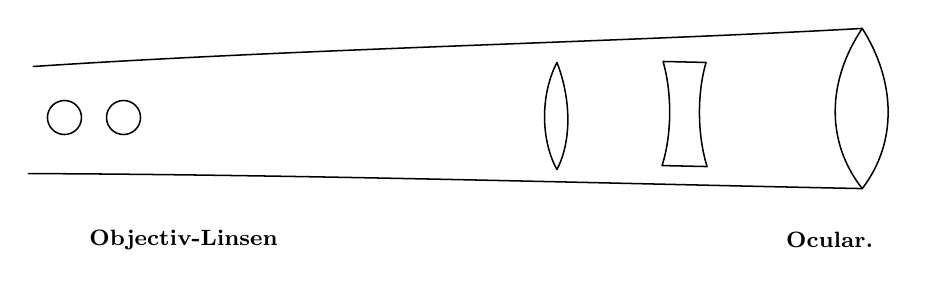
\begin{tikzpicture}[x=.005in,y=-.005in,line width=.55pt,line cap=round,line join=round]
\draw (42,71) .. controls (315,53) and (620,47) .. (870,33);
\draw (37,178) .. controls (315,179) and (620,188) .. (870,193);
\draw (870,33) .. controls (903,85) and (906,146) .. (870,193)
  .. controls (833,146) and (835,85) .. (870,33);
\draw (565,67) .. controls (578,100) and (581,143) .. (565,174)
  .. controls (549,145) and (548,100) .. (565,67);
\draw (671,66) -- (714,67) .. controls (705,97) and (705,139) .. (715,171)
  -- (670,170) .. controls (680,139) and (680,97) .. (671,66);
\draw (73,122) circle[radius=17];
\draw (132,122) circle[radius=17];
\node[anchor=west,font=\footnotesize\bfseries] at (88,244) {Objectiv-Linsen};
\node[anchor=west,font=\footnotesize\bfseries] at (784,244) {Ocular.};
\end{tikzpicture}%
}

\begin{center}
[15.]\par\medskip
\textbf{\textsc{Gauss} an \textsc{Schumacher}.\quad Göttingen, 9. October 1840.}\par\medskip
\rule{.84\linewidth}{.4pt}\par\smallskip
{\footnotesize [Briefwechsel zwischen \textsc{Gauss} und \textsc{Schumacher} III, Altona 1861, S. 406, 407.]}\par\smallskip
\rule{.84\linewidth}{.4pt}
\end{center}
\noindent . . . . . . . . . . . . . . . . . . . . .\par
\noindent\hspace*{\parindent}Da ich eine Gelegenheit habe, ein dialytisches Fernrohr zu acquiriren, wenn ich, ohne es vorher gesehen zu haben (es ist noch in Wien), es übernehmen will, da der Besteller es jetzt nicht braucht, so würde mir angenehm sein, wenn Sie mir vorher von dem Ihrigen noch eine nähere Mittheilung machen wollen. Ich hatte bisher geglaubt, dass es nur zwei (von einander getrennte Linsen) habe, und theoretische Betrachtungen ergeben, dass dann das ganze Princip, nichts taugen würde, d. i. dass gar kein reiner Achromatismus dann möglich ist. Allein nach Einsicht eines übrigens höchst oberflächlichen Aufsatzes von \textsc{Jaquier} in \textsc{Baumgartners} Zeitschrift[*)]\begingroup\renewcommand{\thefootnote}{}\footnotetext{[*) Gemeint ist offenbar der oben S. 155 genannte Aufsatz von \textsc{Jacquin}.]}\endgroup\ scheint es, dass immer 3 Objectivlinsen da sind. Dann ist allerdings Achromatismus möglich, wenn sie \textls[120]{alle drei} getrennt sind.
\begin{center}\DioptrikLetterFifteenDiagram\end{center}
\noindent\hspace*{\parindent}Aber nach der Beschreibung scheint es, dass die zweite und dritte Linse nahe bei einander stehen, und dann muss ich wieder den vollkommenen Achromatismus bezweifeln. Gründlich a priori urtheilen kann ich freilich nicht, ohne genaue quantitative Data über die drei Brennweiten der drei Linsen und die beiden Distanzen, und so erlaube ich mir kein Urtheil darüber, in wie fern die Unvollkommenheit, welche die Theorie andeutet, in der Ausübung noch fühlbar ist. Unbeschadet dieser Unvollkommenheit könnte ein solches Fernrohr Doppelsterne im \textls[120]{Centrum des Gesichtsfeldes} ganz vortrefflich zeigen, und doch den \textls[120]{andern} Bedingungen, welche man an ein Fernrohr macht, nicht genügen. Betrachten Sie also doch gefälligst einmal z. B. Castor \textls[120]{weit vom Centrum} des Gesichtsfeldes, ob der Zwischenraum noch ganz rein erscheint?, oder ob ein Planet \textls[120]{weit vom Centrum} ganz
\par\clearpage\SourceLeaf{164}\HistoricalHead{159}{R}{GAUSS, SCHUMACHER.}
\noindent farbenfrei erscheint. \textsc{Sartorius} hat ein dialytisches Fernrohr von \textsc{Plössl}, ich glaube für 570 fl. erhalten, womit er \textls[120]{gar nicht zufrieden} ist. Die Venus zeigte stark Farben und das Gesichtsfeld sei ganz ungebührlich klein, verhältnissmässig zu den vorhandenen Vergrösserungen. Beides würde mit den Mängeln, welche die Theorie andeutet (so weit es wie gesagt, ohne genaue quantitative Data möglich ist) übereinstimmen. . . . . . . .
\begin{center}
[16.]\par\medskip
\textbf{\textsc{Schumacher} an \textsc{Gauss}.\quad Altona, 12. October 1840.}\par\medskip
\rule{.80\linewidth}{.4pt}\par\smallskip
{\footnotesize \{Briefwechsel zwischen \textsc{Gauss} und \textsc{Schumacher} III, Altona 1861, S. 409.]}\par\smallskip
\rule{.80\linewidth}{.4pt}
\end{center}
\noindent \{. . . . . . . . . . . . . . . . . . . . .\par
\noindent\hspace*{\parindent}Mit den dialytischen Fernröhren ist es mir so gegangen. Ein kleines von etwa 57 Millimeter Öffnung, welches ich von \textsc{Plössl} erhielt, ist vortrefflich, und thut vielleicht etwas mehr als die \textsc{Fraunhofer}schen von $2\frac{1}{2}$ Fuss Brennweite\textsuperscript{*)}.\begingroup\renewcommand{\thefootnote}{}\footnotetext{*) Es zeigt $\varepsilon$ Bootis scharf getrennt.}\endgroup\ Nachher verschrieb ich mir ein grösseres von 34 oder 37 Linien Öffnung (nach dem Preise wohl dasselbe, das \textsc{Sartorius} hat), das gar nicht gut ausfiel. 3 oder 4 kleinere, die ich für Freunde verschrieb, waren sehr mittelmässig, ebenso ein paar von derselben Grösse (57 Millimeter), die ich in Petersburg gesehen habe. Jetzt habe ich wieder eines derselben Gattung bekommen, das seit ein paar Jahren bestellt ist, aber für wen, weiss ich nicht mehr, und das in optischer Hinsicht \textls[120]{besser} als mein Fernrohr ist, obgleich die Metall-Arbeit daran schlechter ist. Ich habe gleich \textsc{Plössl} gefragt, für wen es sei, da ich in der langen Zeit die Bestellung vergessen habe. Seit 4 oder 5 Monaten warte ich vergebens auf Antwort, und glaube also es Jedem, der es wünscht, abgeben zu können. Wollen Sie durchaus ein dialytisches Fernrohr, so würde ich sehr zu \textls[120]{diesem} rathen. Der Preis ist 140 fl. Conventions-Münze (20 fl.-Fuss) und etwa 7 Mark für den Transport. Die beiden mittleren Linsen sind in allen \textsc{Plössl}schen Fernröhren fest verbunden, und sogar durch eine Mastix ähnliche Substanz an einander gekittet\textsuperscript{**)}.\begingroup\renewcommand{\thefootnote}{}\footnotetext{**) Nach \textsc{Jacquins} mündlicher Äußerung.}\endgroup\ \textsc{Steinheil}
\par\clearpage\SourceLeaf{165}\HistoricalHead{160}{L}{PHYSIK.\quad BRIEFWECHSEL.}
\noindent hatte hier ein Fernrohr, bei dem die Entfernung der mittleren Linsen sowohl unter sich, als von der Objectivlinse verändert werden konnte, und meinte, wenn ich recht erinnere, durch Bewegung der einen mittleren Linse die Aberration wegen der Kugelgestalt, durch Bewegung der andern mittleren Linse den Achromatismus corrigiren zu können. Die von Ihnen angegebene Probe habe ich wegen des ungünstigen Wetters noch nicht machen können, werde aber sogleich, wenn sie gemacht ist, darüber berichten.

Ein sehr kleines Gesichtsfeld haben alle dialytischen Fernrohre, die ich gesehen habe, wahrscheinlich um die.\ Verzerrung des Bildes an den Gränzen nicht so merkbar zu machen. Alle haben \textls[120]{eine} einfache Objectivlinse, und in der Mitte \textls[120]{zwei} fest verbundene Linsen, an denen in allen Fällen nichts unter sich zu verändern ist. Bei einem einzigen Fernrohre war ihre Lage gegen die Objectivlinse durch 3 Schrauben, natürlich in engen Gränzen, zu ändern. . . . . . . .\}
\begin{center}
[17.]\par\medskip
\textbf{\textsc{Gauss} an \textsc{Gerling}.\quad Göttingen, 24. October 1840.}
\end{center}
\noindent . . . . . . . . . . . . . . . . . . . . .\par
\noindent\hspace*{\parindent}Theoretische Untersuchungen über die dialytischen Fernröhre scheinen mir zu ergeben, dass diese ganze Einrichtung nicht viel taugt. Es ist unmöglich, vollkommenen Achromatismus damit zu erreichen. \textls[120]{Nur im Centrum des Gesichtsfeldes} können die Bilder farbenfrei sein, nicht aber in beträchtlicher Entfernung vom Centrum. Daher scheint auch die Klage ihren Grund zu haben, dass diese Fernröhre ein ganz ungebührlich kleines Gesichtsfeld haben. In der That, bei grossen Gesichtsfeldern würde dieser der Theorie nach unvermeidliche Fehler gar zu merklich hervortreten. Ich selbst habe nie eins gesehen, vielleicht erhalte ich aber bald ein solches. . . . . . . . . .
\clearpage\endgroup
